% Options for packages loaded elsewhere
\PassOptionsToPackage{unicode}{hyperref}
\PassOptionsToPackage{hyphens}{url}
%
\documentclass[
  a4paper,
]{article}
\usepackage{amsmath,amssymb}
\usepackage{lmodern}
\usepackage{ifxetex,ifluatex}
\ifnum 0\ifxetex 1\fi\ifluatex 1\fi=0 % if pdftex
  \usepackage[T1]{fontenc}
  \usepackage[utf8]{inputenc}
  \usepackage{textcomp} % provide euro and other symbols
\else % if luatex or xetex
  \usepackage{unicode-math}
  \defaultfontfeatures{Scale=MatchLowercase}
  \defaultfontfeatures[\rmfamily]{Ligatures=TeX,Scale=1}
\fi
% Use upquote if available, for straight quotes in verbatim environments
\IfFileExists{upquote.sty}{\usepackage{upquote}}{}
\IfFileExists{microtype.sty}{% use microtype if available
  \usepackage[]{microtype}
  \UseMicrotypeSet[protrusion]{basicmath} % disable protrusion for tt fonts
}{}
\makeatletter
\@ifundefined{KOMAClassName}{% if non-KOMA class
  \IfFileExists{parskip.sty}{%
    \usepackage{parskip}
  }{% else
    \setlength{\parindent}{0pt}
    \setlength{\parskip}{6pt plus 2pt minus 1pt}}
}{% if KOMA class
  \KOMAoptions{parskip=half}}
\makeatother
\usepackage{xcolor}
\IfFileExists{xurl.sty}{\usepackage{xurl}}{} % add URL line breaks if available
\IfFileExists{bookmark.sty}{\usepackage{bookmark}}{\usepackage{hyperref}}
\hypersetup{
  pdftitle={Sensorimotor Learning in Virtual Environments},
  pdfauthor={Spencer R. Wilson},
  hidelinks,
  pdfcreator={LaTeX via pandoc}}
\urlstyle{same} % disable monospaced font for URLs
\usepackage[margin=30mm]{geometry}
\usepackage{graphicx}
\makeatletter
\def\maxwidth{\ifdim\Gin@nat@width>\linewidth\linewidth\else\Gin@nat@width\fi}
\def\maxheight{\ifdim\Gin@nat@height>\textheight\textheight\else\Gin@nat@height\fi}
\makeatother
% Scale images if necessary, so that they will not overflow the page
% margins by default, and it is still possible to overwrite the defaults
% using explicit options in \includegraphics[width, height, ...]{}
\setkeys{Gin}{width=\maxwidth,height=\maxheight,keepaspectratio}
% Set default figure placement to htbp
\makeatletter
\def\fps@figure{htbp}
\makeatother
\setlength{\emergencystretch}{3em} % prevent overfull lines
\providecommand{\tightlist}{%
  \setlength{\itemsep}{0pt}\setlength{\parskip}{0pt}}
\setcounter{secnumdepth}{5}

%% pandoc-fignos: required package
\usepackage[capitalise]{cleveref}
\ifluatex
  \usepackage{selnolig}  % disable illegal ligatures
\fi
\newlength{\cslhangindent}
\setlength{\cslhangindent}{1.5em}
\newlength{\csllabelwidth}
\setlength{\csllabelwidth}{3em}
\newenvironment{CSLReferences}[2] % #1 hanging-ident, #2 entry spacing
 {% don't indent paragraphs
  \setlength{\parindent}{0pt}
  % turn on hanging indent if param 1 is 1
  \ifodd #1 \everypar{\setlength{\hangindent}{\cslhangindent}}\ignorespaces\fi
  % set entry spacing
  \ifnum #2 > 0
  \setlength{\parskip}{#2\baselineskip}
  \fi
 }%
 {}
\usepackage{calc}
\newcommand{\CSLBlock}[1]{#1\hfill\break}
\newcommand{\CSLLeftMargin}[1]{\parbox[t]{\csllabelwidth}{#1}}
\newcommand{\CSLRightInline}[1]{\parbox[t]{\linewidth - \csllabelwidth}{#1}\break}
\newcommand{\CSLIndent}[1]{\hspace{\cslhangindent}#1}

\title{Sensorimotor Learning in Virtual Environments}
\author{Spencer R. Wilson}
\date{\today}

\usepackage[capitalise]{cleveref}
\usepackage{graphicx}
\graphicspath{{/Users/spencerw/Google Drive/motor_control/phd/}}
\usepackage{subfigure}

\begin{document}
\maketitle

\hypertarget{sec:intro}{%
\section{Introduction \& Aims}\label{sec:intro}}

\begin{quote}
\emph{Movement is nothing but the quality of our being.}

--- Sunryu Suzuki, \emph{Zen Mind, Beginner's Mind}
\end{quote}

Hans Moravec's eponymous paradox states that it is easier to generate
artificially intelligent performance on tasks we think of as
intellectually challenging, such as chess, than to provide a machine
with faculties we take for granted, such as movement. For example,
Moravec's Paradox encourages us to not look past the stunningly complex
computations generated by the human motor apparatus. Following Moravec's
suggestion, this work focuses on the human motor system, the most
advanced control apparatus in the known universe.

A recent review corroborates this perspective and provides a clear call
to action:

\begin{quote}
The processes by which biological control solutions spanning large and
continuous state spaces are constructed remain relatively unexplored.
Future investigations may need to embed rich dynamical interactions
between object dynamics and task goals in novel and complex
movements.\textsuperscript{\protect\hyperlink{ref-McNamee2019}{1}}
\end{quote}

Over the last few decades, there has been considerable amount of work
done to untangle the abilities of the motor system to flexibly control
the body including through optimal control
theory\textsuperscript{\protect\hyperlink{ref-Todorov2004}{2}},
reinforcement learning in continuous action
space\textsuperscript{\protect\hyperlink{ref-koberReinforcementLearningRobotics2013}{3}},
and detailed physiological
studies\textsuperscript{\protect\hyperlink{ref-sauerbreiCorticalPatternGeneration2019}{4}}.
However, as the quote above suggests, a holistic understanding of the
computations underlying the generation of skilled movement remains an
open problem. The aim of this thesis is to progress our understanding of
skilled movement by studying the solutions produced by human subjects to
motor tasks in dynamically rich, yet controlled, virtual environments.
Our goal is to reverse-engineer the ability to acquire and perform novel
motor skills. First we define what we mean by the terms \emph{skill},
and \emph{task}.

Humans produce a great variety of movements every day, often without
conscious thought. For example, movements like bringing a cup of coffee
to our lips for a sip are generally out of reach for state-of-the-art
robotic systems. We claim that this ``motor gap'' between biological and
artificial motor systems is due to a lack of \emph{dexterity} in the
latter. Soviet neuroscientist Nikolai Bernstein defined dexterity as the
ability to ``find a motor solution in any situation and in any
condition.''\textsuperscript{\protect\hyperlink{ref-Bernstein1967}{5}}
The crux of this definition is the flexibility of such solutions. This
flexibility, or
robustness\footnote{Kitano defines robustness as ``the maintenance of
  specific functionalities of the system against perturbations, and it
  often requires the system to change its mode of operation in a
  flexible way.'' He claims that robustness requires control,
  alternative mechanisms, modularity and decoupling between high and low
  level variability.}\textsuperscript{\protect\hyperlink{ref-kitanoBiologicalRobustness2004}{6}},
is the ability to optimize internal parameters in response to external
perturbations and adapt to new information to achieve the goals of an
ongoing plan.

While a robot may be able to move a cup of coffee to a precise location
in space, its solution is often found to be brittle in a new context, or
unable to generalize to the movement of new objects. We define a skill
as a behavior that involves dexterity in Bernstein's sense. The use of a
tool such as a screwdriver is an example of a motor skill. We define a
task as the production of skilled movement in a particular context.
Driving a screw in a particular posture using a particular screwdriver
is an example of a task. These concepts will be further formalized in
later chapters.

Human movement is ultimately the result of the activation and
contraction of muscle fibers, and movements lie on a spectrum between
reflexive and volitional. The supramuscular circuitry which determines
the degree of volition we ascribe to movement, where volitional movement
relies on supraspinal (though not necessarily conscious) processes. The
human hand is a unique evolutionary invention that underlies our ability
to perform various skills in a range of tasks-- movements that are
decidedly volitional\footnote{It could be argued that the hand is in
  fact a crucial aspect of humanness. It is thought that the human
  cerebellar and neocortices evolved reciprocally to expand and support
  the computational burden of increasingly complex motor tasks such as
  tool-making and language production. REF?}. The hand is the pinnacle
of dexterity and, as such, it is a fruitful testbed for studying the
computations and circuitry that drive dexterous movement. A detailed
physiological review of the hand and it's relation to skilled movement
is described in \cref{sec:physiology}.

We are more interested in the leveraging the hand as a readout of
flexible motor behavior than we are in the kinematics of hand movement
itself. For this reason, we chose to develop an experimental setup that
is capable of recording directly from muscle activations. We achieve
this through surface electromyography recordings taken from the forearms
controlling subjects' dominant hands. This allows us to track the
sequential selection of muscle these contractions during skill
acquisition and subsequent goal-oriented muscle activations. As we are
interested in subjects' abilities to acquire new skills, we design tasks
that require subjects to use available, but uncommon, motor activations.
We then track the selection and execution of these activation during
virtual tasks. The details of how this is achieved are described in
\cref{sec:experiment}.

how are value computations connected to action and policy selection how
are feedback controllers adapted to motor errors, new environments, how
are they learned as well as combined?

Using data from our experimental setup, we hope to gain an understanding
of how the structure of muscle activation variability in evolves during
skill acquisition and how the motor system constructs skilled movement
through the composition of component muscle coactivations. We believe
that to make progress on these two lines of enquiry we should work to
reconcile the language of the experimental sensorimotor control and
learning community with the language of the control theory and
reinforcement learning community, as each of these communities shares a
common goal of understanding the computation underlying the production
of skilled movement. Here we develop several models in this direction,
as described in \cref{sec:theory}.

\hypertarget{sec:physiology}{%
\section{Physiology of the Skilled Movement}\label{sec:physiology}}

\begin{quote}
\emph{Even a simple movement is a global body event.}

--- Bizzi \& Ajemian, \emph{2020}
\end{quote}

As we hope to make progress engineering naturalistic artificial
movement, it will be beneficial to review what is known about the
biological movement system. Beginning with the architecture of the motor
system and it's relation to dexterity will provide a scaffold on which
we can hang our experimental and theoretical investigations detailed in
\cref{sec:experiment} and \cref{sec:theory}. Specifically, we can use
results from prior physiological investigations to ground our
perspective on the computations relevant to skilled hand movements. We
find that the dexterous solutions produced by the human motor system
rely on a incredibly complex architecture, but one in which a spectrum
of modularity and redundancy appear to be organizing principles.

\hypertarget{motor-units-to-muscles}{%
\subsection{Motor Units to Muscles}\label{motor-units-to-muscles}}

Muscles are composed of fibers which contract due to chemical gradients
produced at the neuromuscular junction by action potentials emanating
from alpha-motoneurons (AMN) in the ventral horn of the spinal cord. The
quantum of motor output is the motor unit (MU), which is defined as a
single motoneuron axon and the set of junctions its axon branches form
with one or more muscle fibers. The innervation ratio of a particular
muscle unit is the number of junctions it innervates. In muscles of the
arm, the number of MUs and their innervation ratios each range from tens
to hundreds per muscle and per motor unit, respectively, decreasing as
muscles become more distal.

The MU thus provides the motor system with spatial redundancy at the
muscle level: multiple muscle fibers contract due to a single AMN spike,
and multiple AMNs may overlap in their innervations. The forces produced
by motor units span several orders of magnitude, though most units
produce very small forces. Here we find temporal redundancy: in order to
produce movements, MUs combine to generate a range of
forces\textsuperscript{\protect\hyperlink{ref-fuglevandMechanicalPropertiesNeural2011}{7}}.

Since the innervation ratios of muscles in the forearm and hand are
relatively small compared to more proximal muscles (which contain
thousands of MUs), the logarithmic recruitment and redundancy of motor
units enables the hand to produce movements with very fine
spatiotemporal resolution. Paradoxically, however, the well-known
signal-dependent noise in models of motor output has been found to be
higher for hand muscles than for more proximal muscles, likely due to
small numbers of motor units compare to larger
muscles\textsuperscript{\protect\hyperlink{ref-fuglevandMechanicalPropertiesNeural2011}{7},\protect\hyperlink{ref-harrisSignaldependentNoiseDetermines1998}{8}}.

Muscle fibers are contained within muscle compartments, and each muscle
may have one or more compartments. The fingers of the hand are extended
by the extensor digitorum (ED) which contains four compartments, one for
each of the tendons the muscle produces. Each tendon connects to the
three metaphalangeal joints of each digit. The fingers are flexed by two
muscles, the flexor digitorum superficialis (FDS) and the flexor
digitorum profundus (FDP). Like the ED, these muscles produce four
tendons, one to each finger from each of their four compartments. As
such, one must coactivate these agonist and antagonist muscles in order
to extend or flex a single finger in
isolation\textsuperscript{\protect\hyperlink{ref-fuglevandMechanicalPropertiesNeural2011}{7}}.
Adduction and Abduction of the fingers is produced by the 19 instrinsic
muscles of the hand, each of which has their origin and insertion points
within the hand
itself\textsuperscript{\protect\hyperlink{ref-vanduinenConstraintsControlHuman2011}{9}}.
The instrinisc muscle tendons form a kind of network around each of the
digits.

The human hand, thumb, and forearm system contains more than 30 muscles
and at least 20 degrees of freedom are theoretically available for
actuation. However, due to biomechanical coupling, the effective degrees
of freedom is presumably less than 20. One study found that tendons of
the fingers are arranged in such a way as to perform a kind of
anatomical computation which expands the mechanical capabilities of the
appendage by sharing force across its tendon
network\textsuperscript{\protect\hyperlink{ref-Valero-Cuevas2007}{10}}.
Such computations embedded in the musculoskeletal structure are
additional complexity when theorizing about neural control of the hand.

We believe this structure exists in order to facilitate the acquisition
of new skills and the generalization of existing skills to new contexts.
While the anatomy of the hand and forearm presents constraints on
movement, the system remains capable of producing a incredible variety
of movement
patterns\textsuperscript{\protect\hyperlink{ref-yanUnexpectedComplexityEveryday2020}{11},\protect\hyperlink{ref-Basmajian1963}{12}}\footnote{In
  a classic study, Basmajian and colleagues showed that it is possible
  to activate single motor units in the thumb abductor.}. The structure
of the neuromuscular system that underlies this variety offers many
clues as to the relevant computations required for dexterous movement.

\hypertarget{coordinative-structures}{%
\subsection{Coordinative Structures}\label{coordinative-structures}}

\begin{quote}
\emph{We have some idea as to the intricate design of the puppet and the
puppet strings, but we lack insight into the mind of the puppeteer.}

--- Bizzi \& Ajemian, \emph{2020}
\end{quote}

Nikolai Bernstein coined the phrase ``the degrees-of-freedom problem''
to describe the challenge the motor system faces in coordinating its
many dimension to achieve a goal. Solving this problem requires
dexterity.\textsuperscript{\protect\hyperlink{ref-Bernstein1967}{5}} As
we have seen, redundancy is present from joints and muscles to motor
units and their upstream synaptic partners. However, rather than asking
how the motor control system deals with this ``problem'' overwhelming
complexity, we might instead question why this complexity is
evolutionarily advantageous at all. What does the availability of this
redundancy afford the motor system? How does this redundancy enable
dexterous movement?

A considerable amount of discussion has focused on the existence of
synergies as a simplifying structure which allows the motor system to
``solve'' the redundancy ``problem''. The term motor synergy can be used
descriptively to describe the spatiotemporal coactivation of muscles
necessary for an ongoing task. Synergetic control implies control in the
space of a low-dimensional set of synergy weights rather than
independent control over the actuator dimensions themselves. The control
dimensions are functionally coupled as a result of synergetic action,
which both simplifies the control task and constrains behavior to the
low-dimensional subspace defined by the synergy
weights\textsuperscript{\protect\hyperlink{ref-merelHierarchicalMotorControl2019}{13}}.
This is what Bizzi and colleagues refer to as ``the puppet's strings''.
The term can also be used as a normative model of motor coordination
which implies a constraint in the dimensionality of the descending
supraspinal control signal, the simplifying movements of the puppeteer.

Many studies have contributed to the concept of synergies as a
hard-wired organizing feature of the motor
system\textsuperscript{\protect\hyperlink{ref-DAvella2003}{14}}.\footnote{I
  should really have more studies here, or a really nice review.}
However, these works tend to extrapolate from non-primate preparations,
particularly in the frog, and use tasks which are inherently
low-dimensional to explain covariance structure in primate and human
kinematic and electromyography
data\textsuperscript{\protect\hyperlink{ref-giszterMotorPrimitivesNew2015}{15},\protect\hyperlink{ref-Gao2017}{\textbf{Gao2017?}}}.
That said, it would be foolish to deny the existence of synergistic
muscle coactivation even at the structural level. Careful studies of
force control by the fingertips present a complex story of
dimensionality of control in this
regime.\textsuperscript{\protect\hyperlink{ref-raczSpatiotemporalAnalysisReveals2013}{16}}
Constraints exist in the architecture of the hand as well as its control
system, though we maintain that concept of synergies, especially in the
context of dexterous movement, is often presented as an
oversimplification rather than a mere simplification. We believe the
story of the hand is more complex.

Studies have attempted to quantify the number of effective degrees of
freedom of the hand with various methods. This has primarily been taken
to be the number of linear features which contain a desired level of the
original signal variance, where the signal is the joint angles of the
hand engaged in various
behaviors\textsuperscript{\protect\hyperlink{ref-Ingram2009}{17},\protect\hyperlink{ref-TodorovDimensionality2005}{18}}.
These methods have resulted in roughly 8 linear features of hand
kinematics to solve a variety of tasks, with subtleties found in
inter-task and inter-subject variations.\^{}{[}It has been argued that
the motor repertoire is hardly high-dimensional when compared to the
dimensionality of the visual feature extraction
system\textsuperscript{\protect\hyperlink{ref-yanUnexpectedComplexityEveryday2020}{11}}.
A recent study found that low-variance linear, kinematic components
displayed significantly higher correlation within condition (e.g.~grasp
of a specific object) than across condition. This suggests that these
components carry task-dependent information rather than
condition-independent, task-irrelevant
noise\textsuperscript{\protect\hyperlink{ref-yanUnexpectedComplexityEveryday2020}{11}}.
This suggests that the control of the hand is more nuanced than a set of
fixed synergies.

What Bizzi and colleagues call ``the problem of supraspinal pattern
formation''--how synergies are activated through time-- we argue, in the
context of hand control, is not simplified by the existence of
hard-wired or soft-wired
synergies\textsuperscript{\protect\hyperlink{ref-bizziMotorPlanningExecution2020}{19}}.
The CNS produces control signals in a range of contexts and in response
to continually changing task demands. Rather than the CNS ``simplifying
movement'' through synergetic action, it is more likely that hand
synergies fall out of a optimization strategy which trades off effort
and accuracy where effort may, in part, correspond to independent
control of individual control dimensions. If we limit ourselves to
synergetic control, then we have simply passed the problem to a
lower-dimensional one of the same fundamental nature. Neural control of
the hand likely contains a spectrum of modularity in order to maintain
its role as a flexible instrument. Synergetic action is one end of this
spectrum resulting from the computation and structure of the human
movement machine.

\hypertarget{fractionating-structures}{%
\subsection{Fractionating Structures}\label{fractionating-structures}}

At the other end of the spectrum, years of research has contributed to a
more complex picture of hand function which embraces non-synergistic
movement\textsuperscript{\protect\hyperlink{ref-lemon1993}{20}--\protect\hyperlink{ref-lemon2008}{22}}.
The key insight of the work is that while ``the organization of the
spinal cord is based on relatively rigid muscular modes, a mechanism to
fractionate this is of particular importance for the muscles of the
hands and digits which may need to be employed in a variety of flexible
associations during voluntary movements.'' Careful anatomical work has
shown how monosynaptic corticospinal, or corticomotoneuronal (CM),
connections provide such fractionation in primates which use tools
requiring
dexterity\textsuperscript{\protect\hyperlink{ref-lemonStartingStoppingMovement2019}{23}}.
M connections are specific to the primate corticospinal tract and
specific to distal muscles of the hands and arm. It appears that the
rodent CST contains CM connections until they recede around P10 at which
point they
recede\textsuperscript{\protect\hyperlink{ref-kawasawa2017}{24},\protect\hyperlink{ref-murabe2018}{25}}.

Just as many muscle fibers may be innervated by a single AMN, up to
thousands of neurons contact single AMNs through CM connections or a
variety of spinal interneuron circuits. The hallmark of CM connections
is their influence over multiple muscle compartments as well as multiple
muscles, though typically agonist or antagonist
sets\textsuperscript{\protect\hyperlink{ref-cheneyFunctionalClassesPrimate1980}{26}}.
This may seem counter-intuitive as a means to produce individuated
movement, but experimental evidence in primates has show that the
convergence of many CM collateral fibers onto single AMNs driving the
distal muscles in particular can produce a fine grading of activity over
motor units driving the distal joints. CM cells also appear to play a
role in the inhibition of antagonist muscles prior to contractions
required for
movement.\textsuperscript{\protect\hyperlink{ref-griffinMotorCortexUses2020}{27}}
These findings confirm theories about the excitatory and inhibitory role
of these connection dating back decades, and combine to suggest that
variables encoded in cortical ensembles are more complex than kinematics
or dynamics
alone.\textsuperscript{\protect\hyperlink{ref-cheneyFunctionalClassesPrimate1980}{26}}.

The CM tract thus acts in coordination with synergistic muscle
activations of the hand to achieve control that is balanced between
modularity and flexibility. Findings suggest that there is a bipartite
structure in human motor cortex driving dexterous control of the distal
part of the upper limb which, it has been suggested, evolved under
pressure to quickly generalize between tasks. This work argues that
these two streams of hand control, namely ``fractionated'' and
``synergistic'' control, may interact to produce versatility, and
balancing these subsystems may be a key part of the optimization
function when learning new
skills\textsuperscript{\protect\hyperlink{ref-Rathelot2009}{28}--\protect\hyperlink{ref-Takei2017}{30}}.
This dualism is likely not rigidly dichotomous, but rather a spectrum of
overriding fractionation (so-called ``New M1'') atop a phylogenetically
older system of synergistic
action\textsuperscript{\protect\hyperlink{ref-dumCorticospinalSystemStructural2011}{31}}.
Griffin and colleagues found that CM cells are functionally tuned to a
muscle's mode of activity (agonist, antagonist, fixator) to ``bypass
spinal cord mechanisms and sculpt novel patterns of motor output that
are essential for highly skilled
movements''.\textsuperscript{\protect\hyperlink{ref-griffinCorticomotoneuronalCellsAre2015}{29}}

The degree to which fractionation of movement is learned is unknown.
Skilled piano performers have been found to exhibit a higher degree of
independent movement among the fingers compared to control participants.
Control groups displayed a hierarchical, presumably lower dimensional,
organization of finger movement patterns while pianists showed distinct
but individuated movement
patterns\textsuperscript{\protect\hyperlink{ref-furuyaFlexibilityMovementOrganization2013}{32}}.
These results are imply that with skilled practice humans can produce
finer and more independent movements of the fingers, and construct
bespoke coactivations to solve specific goals. Similarly, studies have
found that coherence between the index finger and thumb is greater on
the dominant hand. This might imply a developmental lateralization, but
use-dependent plasticity due to greater precision grip behavior of the
dominant hand is also a viable
explanation\textsuperscript{\protect\hyperlink{ref-fuglevandMechanicalPropertiesNeural2011}{7}}.

The concept of a balanced control may prove to be a fruitful direction
for theoretical work on dexterous motor control, the goal being to
construct a model which takes into account this spectrum of
individuation into account. The experimental challenge is to identify
tasks which ostensibly require the direct descending connections to
fractionate learned synergies. There is work suggesting that CM
connections synapse primarily on low threshold, low force motor units
that are recruited first. This would imply a difference in synergy
fractionation at lower force as opposed to higher force. This can be
tested easily by including a force parameter in a hand control task. The
hypothesis stemming from the previously described work is that CM
connections override the ``consolidated'' patterns putatively generated
via spinal interneuron circuitry.

\hypertarget{supraspinal-motor-maps}{%
\subsection{Supraspinal Motor Maps}\label{supraspinal-motor-maps}}

It is known from recent work that primary motor cortex (M1) is not an
isolated movement-generating dynamical system, but rather a node in the
network of a feedback-modulated, distributed movement machine. This is
reflected in recent work in the rodent which suggests that task-relevant
movement depends on these network
connections.\textsuperscript{\protect\hyperlink{ref-sauerbreiCorticalPatternGeneration2019}{4}}
This finding is relevant for our purposed as it demonstrates a
fundamental function for cortical input as opposed to a specific
substructure of motor cortex as detailed above in the primate
literature.

Thinking structural architecture of M1 as an input-driven system with
outputs along a spectrum of modularity from synergistic to fractionated,
we can then ask what kind of functional architecture might have evolved
in the neuromuscular controller? Graziano and colleagues found that
500ms electrical stimulation to M1 reliabaly produced stereotyped
movements in primates, shown in
\cref{fig:rathelot_graziano}\textsuperscript{\protect\hyperlink{ref-grazianoORGANIZATIONBEHAVIORALREPERTOIRE2006}{33}}.
These movements appeared to produce goal-oriented actions pulled out of
other contexts such as bringing food to the mouth, and seemed to be
arranged on the cortical sheet topographically in terms of spatial
endpoints rather than as a homonculus. Graziano refers to this as the
cortical ``action map'', that these stimulations tapped into the control
mechanisms of the primate's motor
system\textsuperscript{\protect\hyperlink{ref-grazianoIntelligentMovementMachine2009}{34}}.

\begin{figure}
\hypertarget{fig:rathelot_graziano}{%
\centering
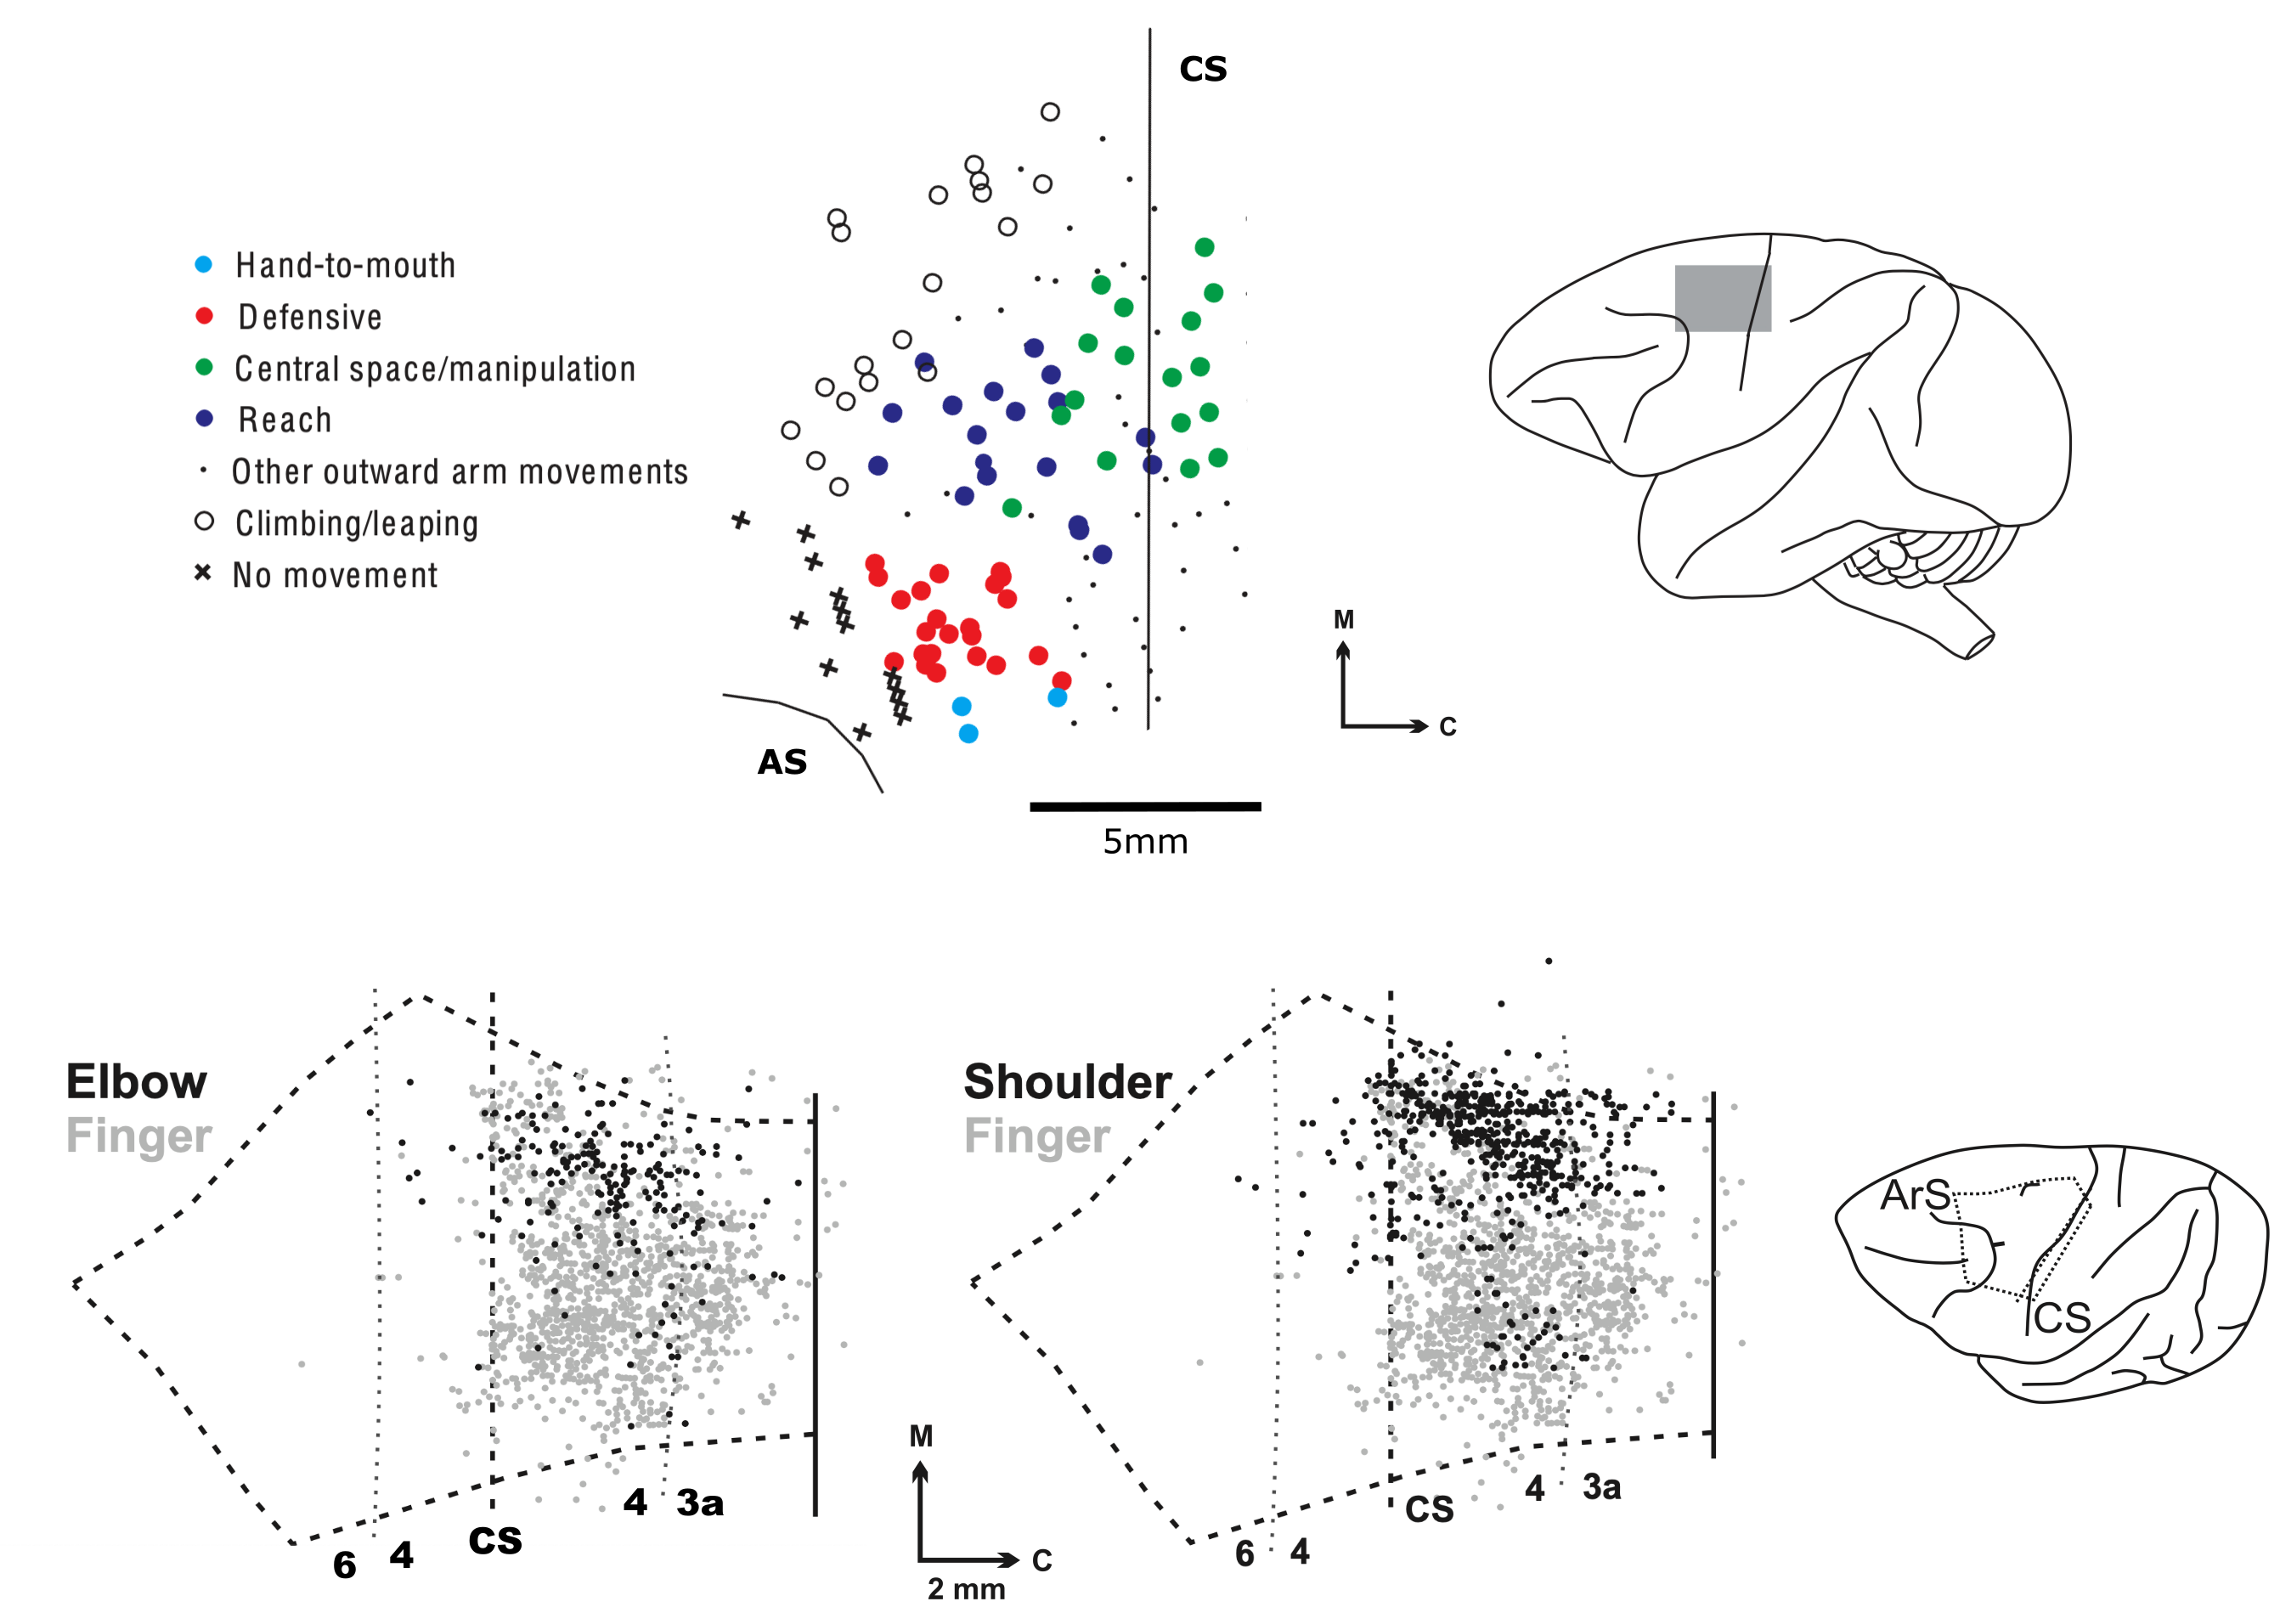
\includegraphics{images/physiology/rathelot_graziano.png}
\caption{Similarities between electrical stimulation on behavorial
timescales and rabies tracing identification of CM cells. CM cells are
largely confined to the caudal half of M1, while this region tends to
evokes complex manipulatory movements when electrically stimulated. (Top
Left) Corticomotoneuronal (CM) cells traced using rabies from muscles of
the elbow and finger. (Top Right) CM cells traced using rabies from
muscles of the shoulder and finger. (Bottom) Complex movements evoked by
500ms electrical stimulation pulse trains. \emph{Adapted from Graziano
2005 and Rathelot 2009}}\label{fig:rathelot_graziano}
}
\end{figure}

Recent work identifying movement syllables on a behaviorally relevant
timescale has a similar flavor. Along with behavioral syllables, the
motor map concept posits the idea that M1 might be looked at like a
field of feedback control microcircuits, integrating and transforming
inputs, both internal and external, to sculpt ongoing
movement.\textsuperscript{\protect\hyperlink{ref-wiltschkoMappingSubSecondStructure2015}{35}}
This is in accordance with the idea that there is a structural hierarchy
in M1 covering a spectrum of movement modularity. These ideas together
form a picture of the motor system as a structural scaffold upon which
behaviorally relevant feedback mappings from cortex to the spinal cord
are continuously activated and modulated based on information and
estimates about the periphery. In this view, the encoded variables of
interest depend on the goals, context, and perturbations of the intended
movement. Graziano writes:

\begin{quote}
``The usefulness of a feedback-dependent mapping from cortex to muscles
is that it can in principle allow neurons in motor cortex to control a
diversity of movement variables, such as direction, speed, hand
position, or posture that transcend a fixed pattern of muscle
activation. If the network receives feedback information about a
specific movement variable, then it can learn to control that
variable.''
\end{quote}

Muscle activity is, in a sense, a readout from a network transforming
state-dependent inputs into movement goals. Rather than playing chords,
the motor system is improvisational jazzmaster. The movement machine
wields its complexity to construct a movement fit to purpose, to suit
its context and the information it receives. Rather than choosing muscle
patterns in reconfigurable blocks, it creatively constructs and sculpts
movements. That is, the hierarchy of the motor system is not rigidly
organized around a particular set of variables. Many loops exist
connecting cortex with the spinal cord, the cerebellum, the basal
ganglia, and the sensorimotor periphery. Each of these loops contributes
information to flexible activate the relevant action maps. Prevailing
theory suggests that cerebellar loops provide predictive state
information while basal gangliar loops provide state and/or action value
information.

The movement machine reasons in the space of feedback control systems
and their ensuing trajectories. The phenomenal thing about the motor
system is that it is able to tune itself rapidly with both
high-dimensional sensory inputs and sparse reward
signals\textsuperscript{\protect\hyperlink{ref-bahlNeuralDynamicPoliciesfor2020}{36},\protect\hyperlink{ref-ijspeertDynamicalMovementPrimitives2013}{37}}.
This has some precedence in the literature and will be discussed further
in \cref{sec:theory}. This section has attempted to illustrate the
complexity of the motor control system specifically with regard to
dexterous control of the hand, with an eye toward experimental and
theoretical avenues for exploration. The goal is to build and test a
theoretical scheme for aspects of the compositional nature of the neural
hand controller.

\hypertarget{sec:experiment}{%
\section{Experimental Methods}\label{sec:experiment}}

\hypertarget{sec:data}{%
\section{Data Analysis}\label{sec:data}}

\hypertarget{sec:theory}{%
\section{Theory}\label{sec:theory}}

\hypertarget{sec:next_steps}{%
\section{Next Steps}\label{sec:next_steps}}

\newpage

\hypertarget{bibliography}{%
\subsection*{Bibliography}\label{bibliography}}
\addcontentsline{toc}{subsection}{Bibliography}

\hypertarget{refs}{}
\begin{CSLReferences}{0}{0}
\leavevmode\hypertarget{ref-McNamee2019}{}%
\CSLLeftMargin{1. }
\CSLRightInline{McNamee, D. \& Wolpert, D. M. Internal {Models} in
{Biological Control}. \emph{Annual Review of Control, Robotics, and
Autonomous Systems} \textbf{2}, 339--364 (2019).}

\leavevmode\hypertarget{ref-Todorov2004}{}%
\CSLLeftMargin{2. }
\CSLRightInline{Todorov, E. Optimality principles in sensorimotor
control. \emph{Nature Neuroscience} \textbf{7}, 907--915 (2004).}

\leavevmode\hypertarget{ref-koberReinforcementLearningRobotics2013}{}%
\CSLLeftMargin{3. }
\CSLRightInline{Kober, J., Bagnell, J. A. \& Peters, J. Reinforcement
learning in robotics: {A} survey. \emph{The International Journal of
Robotics Research} \textbf{32}, 1238--1274 (2013).}

\leavevmode\hypertarget{ref-sauerbreiCorticalPatternGeneration2019}{}%
\CSLLeftMargin{4. }
\CSLRightInline{Sauerbrei, B. A. \emph{et al.} Cortical pattern
generation during dexterous movement is input-driven. \emph{Nature}
(2019)
doi:\href{https://doi.org/10.1038/s41586-019-1869-9}{10.1038/s41586-019-1869-9}.}

\leavevmode\hypertarget{ref-Bernstein1967}{}%
\CSLLeftMargin{5. }
\CSLRightInline{Bernstein, N. \emph{The coordination and regulation of
movements}. ({Pergamon}, 1967).}

\leavevmode\hypertarget{ref-kitanoBiologicalRobustness2004}{}%
\CSLLeftMargin{6. }
\CSLRightInline{Kitano, H. Biological robustness. \emph{Nature Reviews
Genetics} \textbf{5}, 826--837 (2004).}

\leavevmode\hypertarget{ref-fuglevandMechanicalPropertiesNeural2011}{}%
\CSLLeftMargin{7. }
\CSLRightInline{Fuglevand, A. J. Mechanical properties and neural
control of human hand motor units: {Control} of human hand motor units.
\emph{The Journal of Physiology} \textbf{589}, 5595--5602 (2011).}

\leavevmode\hypertarget{ref-harrisSignaldependentNoiseDetermines1998}{}%
\CSLLeftMargin{8. }
\CSLRightInline{Harris, C. M. \& Wolpert, D. M. Signal-dependent noise
determines motor planning. \emph{Nature} \textbf{394}, 780--784 (1998).}

\leavevmode\hypertarget{ref-vanduinenConstraintsControlHuman2011}{}%
\CSLLeftMargin{9. }
\CSLRightInline{van Duinen, H. \& Gandevia, S. C. Constraints for
control of the human hand: {Control} of the hand. \emph{The Journal of
Physiology} \textbf{589}, 5583--5593 (2011).}

\leavevmode\hypertarget{ref-Valero-Cuevas2007}{}%
\CSLLeftMargin{10. }
\CSLRightInline{Valero-Cuevas, F. J. \emph{et al.} The tendon network of
the fingers performs anatomical computation at a macroscopic scale.
\emph{IEEE Transactions on Biomedical Engineering} \textbf{54},
1161--1166 (2007).}

\leavevmode\hypertarget{ref-yanUnexpectedComplexityEveryday2020}{}%
\CSLLeftMargin{11. }
\CSLRightInline{Yan, Y., Goodman, J. M., Moore, D. D., Solla, S. A. \&
Bensmaia, S. J. Unexpected complexity of everyday manual behaviors.
\emph{Nature Communications} \textbf{11}, 3564 (2020).}

\leavevmode\hypertarget{ref-Basmajian1963}{}%
\CSLLeftMargin{12. }
\CSLRightInline{Basmajian, J. V. Control and {Training} of {Individual
Motor Units}. \emph{Science} \textbf{141}, 440--441 (1963).}

\leavevmode\hypertarget{ref-merelHierarchicalMotorControl2019}{}%
\CSLLeftMargin{13. }
\CSLRightInline{Merel, J., Botvinick, M. \& Wayne, G. Hierarchical motor
control in mammals and machines. \emph{Nature Communications}
\textbf{10}, 5489 (2019).}

\leavevmode\hypertarget{ref-DAvella2003}{}%
\CSLLeftMargin{14. }
\CSLRightInline{D'Avella, A., Saltiel, P. \& Bizzi, E. Combinations of
muscle synergies in the construction of a natural motor behavior.
\emph{Nature Neuroscience} \textbf{6}, 300--308 (2003).}

\leavevmode\hypertarget{ref-giszterMotorPrimitivesNew2015}{}%
\CSLLeftMargin{15. }
\CSLRightInline{Giszter, S. F. Motor primitives{}new data and future
questions. \emph{Current Opinion in Neurobiology} \textbf{33}, 156--165
(2015).}

\leavevmode\hypertarget{ref-raczSpatiotemporalAnalysisReveals2013}{}%
\CSLLeftMargin{16. }
\CSLRightInline{Rácz, K. \& Valero-Cuevas, F. J. Spatio-temporal
analysis reveals active control of both task-relevant and
task-irrelevant variables. \emph{Frontiers in Computational
Neuroscience} \textbf{7}, (2013).}

\leavevmode\hypertarget{ref-Ingram2009}{}%
\CSLLeftMargin{17. }
\CSLRightInline{Ingram, J. N. \& Wolpert, D. M. The statistics of
natural hand movements. \emph{Brain} \textbf{188}, 223--236 (2009).}

\leavevmode\hypertarget{ref-TodorovDimensionality2005}{}%
\CSLLeftMargin{18. }
\CSLRightInline{Todorov, E. \& Ghahramani, Z. Analysis of the synergies
underlying complex hand manipulation. in \emph{The 26th {Annual
International Conference} of the {IEEE Engineering} in {Medicine} and
{Biology Society}} vol. 4 4637--4640 ({IEEE}, 2005).}

\leavevmode\hypertarget{ref-bizziMotorPlanningExecution2020}{}%
\CSLLeftMargin{19. }
\CSLRightInline{Bizzi, E. \& Ajemian, R. From motor planning to
execution: A sensorimotor loop perspective. \emph{Journal of
Neurophysiology} \textbf{124}, 1815--1823 (2020).}

\leavevmode\hypertarget{ref-lemon1993}{}%
\CSLLeftMargin{20. }
\CSLRightInline{Lemon, R. N. Cortical control of the primate hand.
\emph{Experimental Physiology} \textbf{78}, 263--301 (1993).}

\leavevmode\hypertarget{ref-lemon1997}{}%
\CSLLeftMargin{21. }
\CSLRightInline{Lemon, R. N. Mechanisms of cortical control of hand
function. \emph{Neuroscientist} \textbf{3}, 389--398 (1997).}

\leavevmode\hypertarget{ref-lemon2008}{}%
\CSLLeftMargin{22. }
\CSLRightInline{Lemon, R. N. Descending {Pathways} in {Motor Control}.
\emph{Annual Review of Neuroscience} \textbf{31}, 195--218 (2008).}

\leavevmode\hypertarget{ref-lemonStartingStoppingMovement2019}{}%
\CSLLeftMargin{23. }
\CSLRightInline{Lemon, R. \& Kraskov, A. Starting and stopping movement
by the primate brain. \emph{Brain and Neuroscience Advances} \textbf{3},
239821281983714 (2019).}

\leavevmode\hypertarget{ref-kawasawa2017}{}%
\CSLLeftMargin{24. }
\CSLRightInline{Kawasawa, Y. I. \emph{et al.} Control of
species-dependent cortico-motoneuronal connections underlying manual
dexterity. \emph{Science} \textbf{357}, 400--404 (2017).}

\leavevmode\hypertarget{ref-murabe2018}{}%
\CSLLeftMargin{25. }
\CSLRightInline{Murabe, N. \emph{et al.} Higher primate-like direct
corticomotoneuronal connections are transiently formed in a juvenile
subprimate mammal. \emph{Scientific Reports} \textbf{8}, 1--10 (2018).}

\leavevmode\hypertarget{ref-cheneyFunctionalClassesPrimate1980}{}%
\CSLLeftMargin{26. }
\CSLRightInline{Cheney, P. D. \& Fetz, E. E. Functional classes of
primate corticomotoneuronal cells and their relation to active force.
\emph{Journal of Neurophysiology} \textbf{44}, 773--791 (1980).}

\leavevmode\hypertarget{ref-griffinMotorCortexUses2020}{}%
\CSLLeftMargin{27. }
\CSLRightInline{Griffin, D. M. \& Strick, P. L. The motor cortex uses
active suppression to sculpt movement. \emph{Science Advances}
\textbf{6}, eabb8395 (2020).}

\leavevmode\hypertarget{ref-Rathelot2009}{}%
\CSLLeftMargin{28. }
\CSLRightInline{Rathelot, J.-A. \& Strick, P. L. Subdivisions of primary
motor cortex based on cortico-motoneuronal cells. \emph{Proceedings of
the National Academy of Sciences} \textbf{106}, 918--923 (2009).}

\leavevmode\hypertarget{ref-griffinCorticomotoneuronalCellsAre2015}{}%
\CSLLeftMargin{29. }
\CSLRightInline{Griffin, D. M., Hoffman, D. S. \& Strick, P. L.
Corticomotoneuronal cells are "functionally tuned". \emph{Science}
\textbf{350}, 667--670 (2015).}

\leavevmode\hypertarget{ref-Takei2017}{}%
\CSLLeftMargin{30. }
\CSLRightInline{Takei, T., Confais, J., Tomatsu, S., Oya, T. \& Seki, K.
Neural basis for hand muscle synergies in the primate spinal cord.
\emph{Proceedings of the National Academy of Sciences} \textbf{114},
8643--8648 (2017).}

\leavevmode\hypertarget{ref-dumCorticospinalSystemStructural2011}{}%
\CSLLeftMargin{31. }
\CSLRightInline{Dum, R. P. \& Strick, P. L. The {Corticospinal System}:
{A Structural Framework} for the {Central Control} of {Movement}. in
\emph{Comprehensive {Physiology}} ({John Wiley \& Sons, Inc.}, 2011).
doi:\href{https://doi.org/10.1002/cphy.cp120106}{10.1002/cphy.cp120106}.}

\leavevmode\hypertarget{ref-furuyaFlexibilityMovementOrganization2013}{}%
\CSLLeftMargin{32. }
\CSLRightInline{Furuya, S. \& Altenmüller, E. Flexibility of movement
organization in piano performance. \emph{Frontiers in Human
Neuroscience} \textbf{7}, (2013).}

\leavevmode\hypertarget{ref-grazianoORGANIZATIONBEHAVIORALREPERTOIRE2006}{}%
\CSLLeftMargin{33. }
\CSLRightInline{Graziano, M. {THE ORGANIZATION OF BEHAVIORAL REPERTOIRE
IN MOTOR CORTEX}. \emph{Annual Review of Neuroscience} \textbf{29},
105--134 (2006).}

\leavevmode\hypertarget{ref-grazianoIntelligentMovementMachine2009}{}%
\CSLLeftMargin{34. }
\CSLRightInline{Graziano, M. S. A. \emph{The intelligent movement
machine: An ethological perspective on the primate motor system}.
({Oxford University Press}, 2009).}

\leavevmode\hypertarget{ref-wiltschkoMappingSubSecondStructure2015}{}%
\CSLLeftMargin{35. }
\CSLRightInline{Wiltschko, A. B. \emph{et al.} Mapping {Sub}-{Second
Structure} in {Mouse Behavior}. \emph{Neuron} \textbf{88}, 1121--1135
(2015).}

\leavevmode\hypertarget{ref-bahlNeuralDynamicPoliciesfor2020}{}%
\CSLLeftMargin{36. }
\CSLRightInline{Bahl, S., Mukadam, M., Gupta, A. \& Pathak, D. Neural
{Dynamic Policiesfor End}-to-{End Sensorimotor Learning}. 5 (2020).}

\leavevmode\hypertarget{ref-ijspeertDynamicalMovementPrimitives2013}{}%
\CSLLeftMargin{37. }
\CSLRightInline{Ijspeert, A. J., Nakanishi, J., Hoffmann, H., Pastor, P.
\& Schaal, S. Dynamical {Movement Primitives}: {Learning Attractor
Models} for {Motor Behaviors}. \emph{Neural Computation} \textbf{25},
328--373 (2013).}

\end{CSLReferences}

\end{document}
